\chapter*{Введение}
\addcontentsline{toc}{chapter}{Введение}

Методическое пособие описывает основные шаги по разработке программного обеспечения для встраиваемых систем. В качестве целевой платформы используется плата «Багет ПЛК1-01» с установленным микроконтроллером Комдив-МК К5500ВК018, производства ФГУ ФНЦ НИИСИ РАН. В состав К5500ВК018 входит суперскалярное 64-разрядное RISC микропроцессорное ядро с архитектурой КОМДИВ64 (MIPS64-совместимая), включая сопроцессор вещественной арифметики (IEEE754), кэш-память первого уровня (16+16 КБайт), кэш-память второго уровня (128 КБайт), буфер трансляции виртуальных адресов на 64 адреса, контроллер динамической памяти DDR3 с поддержкой DDR3L, восемь таймеров-счетчиков, сторожевой таймер, часы реального времени, два контроллера Ethernet 10/100, контроллеры последовательных интерфейсов UART (5 шт.), I2C (3 шт.), SPI (4 шт.), CAN 2.0 (2 шт.), USB 2.0, контроллер SDHCI. Серийный выпуск начат в 2021 году. 

ПЛК1-01 выполнен в виде печатной платы без корпуса, на которой расположены
соединители для подключения первичного электропитания и внешних устройств, органы
управления (пользовательские кнопки SW1, SW2), светодиодные индикаторы (VD1 –
VD5), перемычки для управления режимами работы ПЛК1-01 (SA4, SA5, SA6, SA7, SA9). 

\begin{center}
	\begin{tabular}{||c | c||}
		\hline
		Назначение & Вывод процессора \\ [0.5ex]
		\hline\hline
		Кнопка SW2 & GPIOD 6 \\
		\hline
		Зелёный светодиод VD2 & GPIOD 4 \\
		\hline
		Жёлтый светодиод VD5 & GPIOD 5 \\
		\hline
	\end{tabular}
\end{center}

Для организации питания часов реального времени (RTC) микроконтроллера
К5500ВК018 при отсутствии основного питания предусмотрена установка
автономного элемента питания – батарейки типа CR2032 +3 В.
Расположение соединителей, органов управления и индикаторов ПЛК1-01
приведено на рисунке \ref{fig:fig1}, назначение выводов на некоторых из разъёмов приведены на рисунке \ref{fig:fig2}.

\begin{center}
	\begin{figure}
		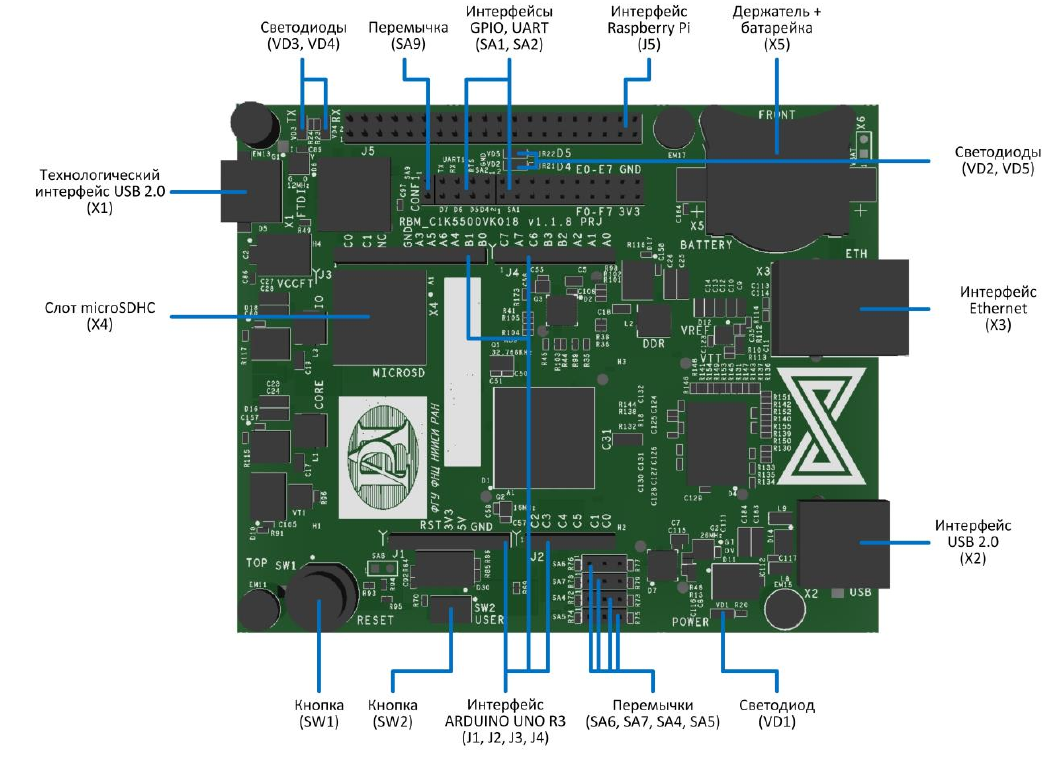
\includegraphics[width=\textwidth]{pic_01}
		\caption{Расположение портов ввода-вывода}
		\label{fig:fig1}
	\end{figure}
\end{center}

\begin{center}
	\begin{figure}
		\centering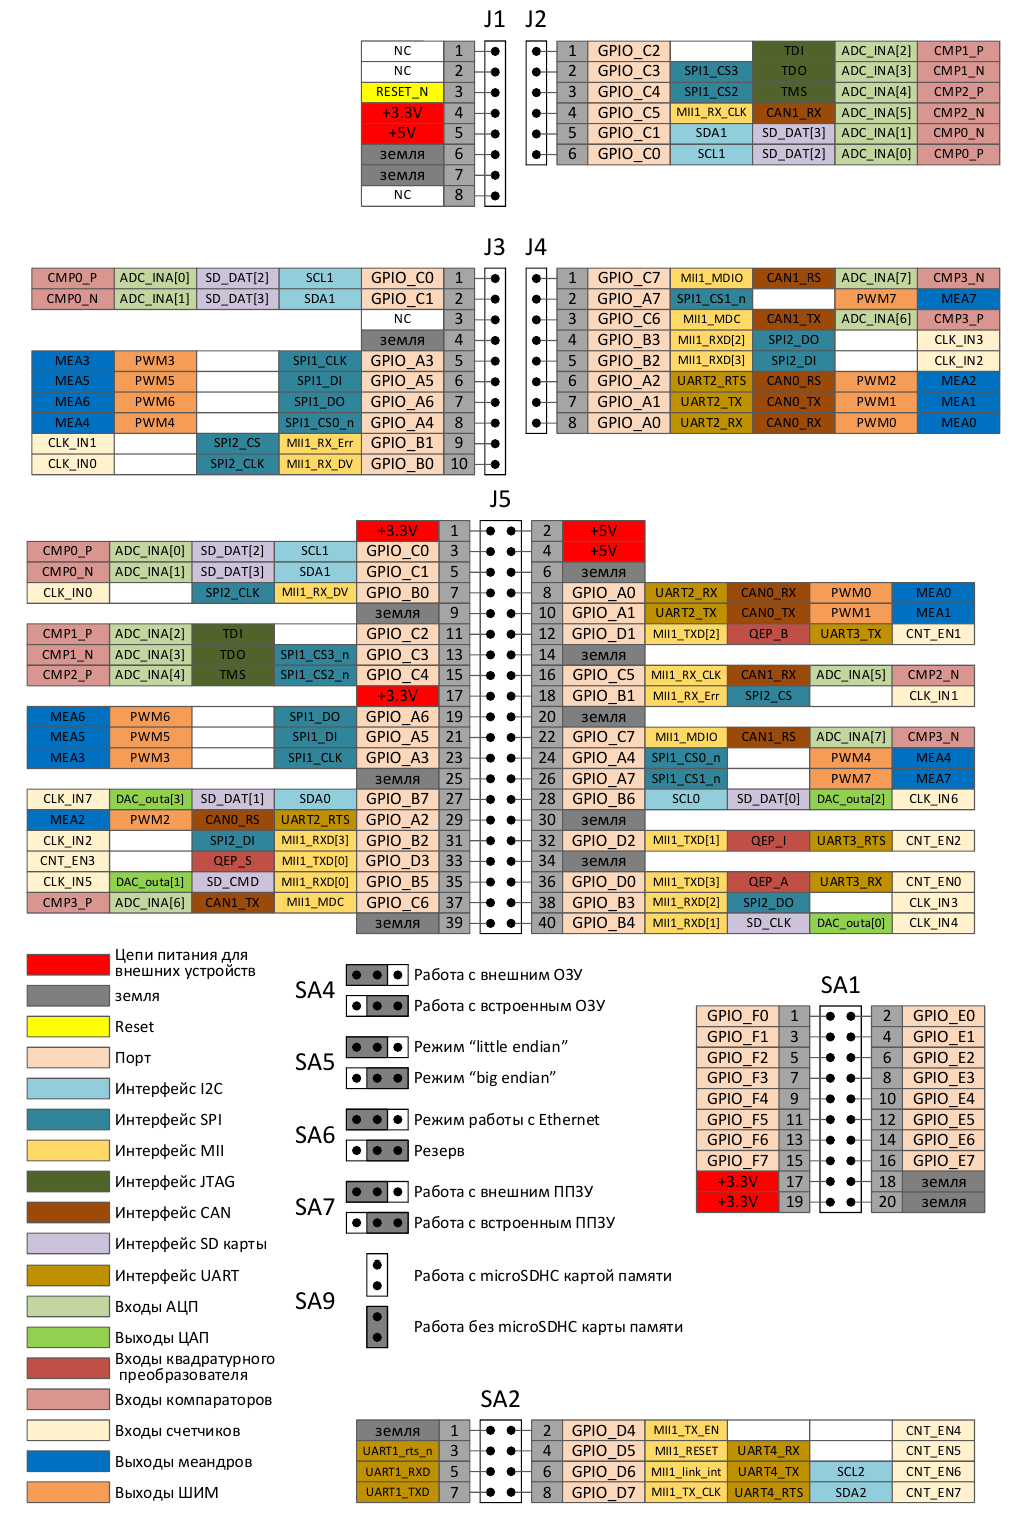
\includegraphics[width=\textwidth]{pic_02}
		\caption{Разводка выводов процессора по разъёмам ввода-вывода}
		\label{fig:fig2}
	\end{figure}
\end{center}

\vspace{10mm}
\section*{Переходная плата}
Для удобства подключения к интерфейсам целевой платы, была разработана переходная плата, с выведенными сигнальными линиями, сгруппированными по интерфейсам (рисунок \ref{fig:fig3}).  

\begin{figure}[hbt!]
	\centering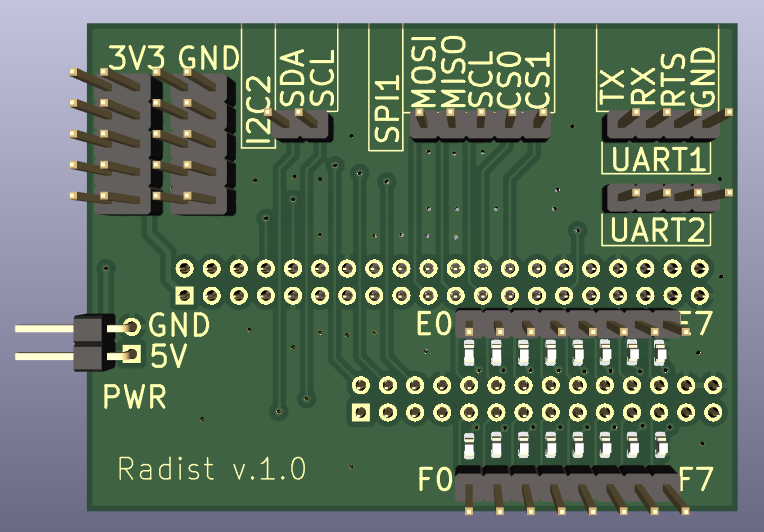
\includegraphics[width=\textwidth]{pic_03}
	\caption{Переходная плата}
	\label{fig:fig3}
\end{figure}

UART2 можно использовать как для работы с интерфейсом UART2, так и для работы с интерфейсом CAN0. Выводы GPIO банков E и F дублируются на светодиоды для отладочных целей. При необходимости, можно подключать к выводам кнопки, или использовать их для формирования управляющих сигналов для модулей. Также обратите внимание, что одна из сигнальных линий I2C интерфейса используется кнопкой SW2 на плате, по этой причине не стоит использовать кнопку при активации этого интерфейса.    


\section*{Как запускается Linux?}
Для запуска ОС Linux в общем случае должны пройти следующие этапы:
\begin{enumerate}
	\item  ROM BOOT — запуск встроенного загрузчика, определяющего источник дальнейшей загрузки. Этот код нельзя исправить его работа и формат образа (заголовки, значение бит и прочее) зависит от производителя.
	
	\item First Stage Bootloader (FSBL) — загрузчик первой ступени, задача этого загрузчика, начальная инициализация процессора, и загрузка пользовательского кода в DDR память. Данный загрузчик опциональный, и у некоторых производителей может отсутствовать. Работает из встроенной RAM памяти процессора.
	
	\item Second Stage Bootloader (SSBL) — это загрузчик второго уровня, задача которого заключается в подготовке системы к запуску ядра Linux, с пользовательскими параметрами (точка монтирования rootfs, скорость работы терминала для логов и прочее). Наиболее распространённый вариант загрузчика Das U-Boot (\href{https://u-boot.readthedocs.io/en/latest/}{https://u-boot.readthedocs.io}). В целевой плате используется другой загрузчик, набирающий популярность — Barebox (\href{https://www.barebox.org/}{https://www.barebox.org/}).
	
	\item Kernel — на этом этапе за работу процессора отвечает ядро операционной системы, происходит финальная конфигурация, активация дополнительный процессорных ядер (если они есть и активирована функция многоядерной поддержки), монтирование rootfs, запуск сервисов и прочее.
\end{enumerate}


\section*{Описание окружения}
Для работы с платой используется виртуальная машина на базе Kubuntu 20.04. На виртуальной машине установлены пакеты для компиляции кода под Linux для MIPS64 архитектуры mips64el-linux-gnu-gcc (C компилятор) и mips64el-linux-gnu-g++ (C++ компилятор), компилятор дерева устройств device-tree-compiler, архив с заголовочными файлами ядра Linux установленного на плате, утилита debootstrap, IDE VSCode и прочие полезные инструменты. 

Имя пользователя \textbf{student} пароль \textbf{usrstudent}. Пользователь поддерживает работу через sudo (получение прав суперпользователя он же администратор).

В конце некоторых работ есть задания для самостоятельного выполнения. При этом есть простые задачи, предполагающие незначительное изменение кода, а также есть помеченные *. Последние выполняются по желанию, при этом нужно быть готовым, что придётся активно пользоваться поиском, и расходовать клетки серого вещества.

\textbf{ВНИМАНИЕ!} Запомните, что далее по тексту, если просят выполнить команду, в начале которой написано \textbf{\$} , значит команду нужно выполнить на целевой плате, а если с \textbf{\#} - в консоли виртуальной машины. При этом \$ или \# писать не нужно! 

Если команда заканчивается символом \verb!\! и на следующей строчке есть запись, то это запись относиться к одной команде, Вы можете записать как видите, так как символ \verb!\! в консоли Linux означает многострочную команду или, опустив символ \verb!\!, продолжить вводить текст приведённый на следующей строке методички.\\

\textbf{Примеры:}

Необходимо ввести в консоли виртуальной машины (ВМ) команду echo Hello:

\begin{lstlisting}[style=bash]
# echo Hello 
\end{lstlisting}

Необходимо ввести в консоли целевой платы команду echo FOOBAR:

\begin{lstlisting}[style=bash]
$ echo FOOBAR
\end{lstlisting}

Необходимо ввести в консоли виртуальной машины (ВМ) очень длинную команду (да-да, вечер не обещает быть томным):

\begin{lstlisting}[style=bash]
# echo \
FOOBAR 
\end{lstlisting}